%\chapterimage{head2.png} % Chapter heading image

\chapter{sheet-1 :Dirac Delta Function}
\label{chapter1.dirac-delta}

\ifpdf
\graphicspath{{Chapter1/figs/}}
\else
\graphicspath{{Chapter1/figs/}}
\fi


	Consider the function $D_\epsilon(x)$ given by
	\begin{eqnarray}
	D_\epsilon(x) &= 
		\begin{cases}
			\frac{1}{\epsilon} \ \ &\text{for} \ \  -\frac{\epsilon}{2} \leq x \leq \frac{\epsilon}{2} \\
			0 \ \ &\text{for} \ \  |x| > \frac{\epsilon}{2} 
		\end{cases}
	\end{eqnarray}
	where $\epsilon$ is a positive parameter. The plot of the function is shown in figure (\ref{fig.cpt1.figure1}).
	
	\begin{figure}
		\centering
		\subfloat[]{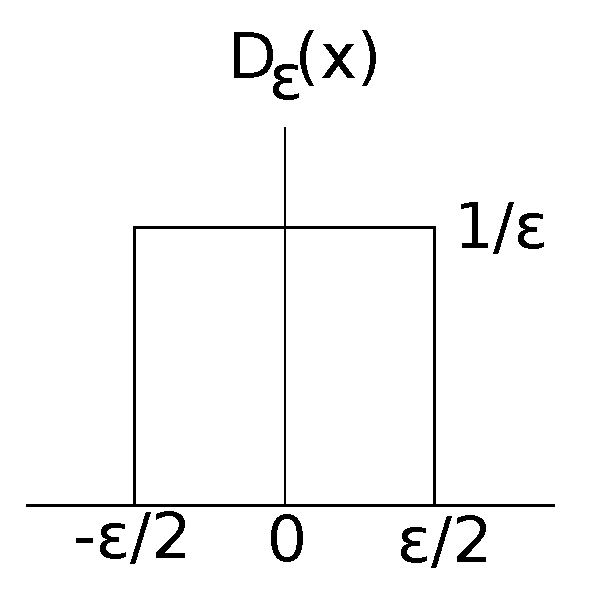
\includegraphics[width=5cm]{delta.pdf}}
		\caption{Dirac Delta Function}
		\label{fig.cpt1.figure1}
	\end{figure}
	
	The integral of the function with respect to $x$ is $1$, i.e.,
	\begin{equation}
		\int_{-\infty}^{\infty} D_\epsilon(x) dx = 1
	\end{equation}
	Now imagine making $\epsilon$ smaller. As we decrease $\epsilon$, the function gets narrower and taller, but the integral of the function(i.e., the area under graph remains constant at the value $1$).
	In the limit $\epsilon \rightarrow 0$, the function $D_\epsilon(x)$ collapses to a single  point $x=0$ and gets infinitely tall. So $\lim\limits_{\epsilon \rightarrow \epsilon} D_\epsilon(x)$ is not a function at all and the procedure of taking the limit is not justified.
	\\
	
	However, we can make the limiting procedure meaningful if multiply $D_\epsilon(x)$ by some well defined function $f(x)$, integrate over $x$ and then take the limit $\epsilon \rightarrow 0 $. consider the integral
	\begin{equation}
		\int_{-\infty}^{\infty} D_\epsilon(x) f(x) dx
	\end{equation}
	where $f(x)$ is a well-defined function. If $\epsilon$ is significantly small, the variation of $f(x)$ over the effective integration interval $[-\epsilon / 2, \epsilon / 2]$ is negligible and $f(x)$ remains practically equal to $f(0)$, therefore,
	\begin{equation}
		\int_{-\infty}^{\infty} D_\epsilon (x) f(x) dx \simeq f(0) \int_{-\infty}^{\infty} D_\epsilon (x) dx = f(0)
	\end{equation}
	The smaller the value of $\epsilon$, the better the approximation. In the limit $\epsilon \rightarrow 0$, the above equation is exact
	\begin{equation}
		\lim\limits_{\epsilon \rightarrow 0}\int_{-\infty}^{\infty} D_\epsilon (x) f(x) dx  = f(0)
	\end{equation}
	Now, we define the delta function by the relation
	\begin{equation}
		\int_{-\infty}^{\infty} \delta(x) f(x) dx \  _=^{def}  \lim\limits_{\epsilon \rightarrow 0}\int_{-\infty}^{\infty} D_\epsilon (x) f(x) dx  = f(0)
	\end{equation}
	This equation is valid for any function $f(x)$ defined at the origin. More generally, $\delta(x - x_0)$ is defined as,
	\begin{equation}
		\int_{-\infty}^{\infty} \delta(x - x_0) f(x) dx \ = f(x_0)
	\end{equation}
	Actually, the integral notation $\int_{-\infty}^{\infty} \delta(x) f(x) dx$ is not justified because $\delta(x)$ is not really a function. Physically, there is no problem since it becomes impossible to distinguish between $D_\epsilon(x)$ and $\delta(x)$ as soon as $\epsilon$ becomes negligible compared to all distances involved in a physical problem. Whenever a mathematical difficulty might arise, all we need to do is to assume that $\delta(x)$ is actually $D_\epsilon(x)$ with $\epsilon$ extremely small but not strictly zero.
	\\
	Formally, we can express $\delta(x)$ as a limit of a square of proper functions : 
	\begin{equation}
		\lim\limits_{\epsilon \rightarrow 0} D_\epsilon(x) \equiv \delta(x)
	\end{equation}
	Here $D_\epsilon(x)$, which is a proper function of $x$ is called the representation of the delta function. One representation is the "square function" given at the beginning. The representation is not unique. There are other functions which approach the delta function when appropriate limits are taken.
	
	\section{Other representation of delta function}
		\begin{enumerate}
			\item 
			Consider the function
			\begin{equation}
				D_\epsilon(x) = \frac{1}{\epsilon \sqrt{\pi}} e^{-x^2/\epsilon^2}  \ \ \ (\epsilon > 0)
				\label{eqn.other-reps-exp}
			\end{equation}
			For each value of the parameter $\epsilon$, this function satisfies
			\begin{equation}
			\int_{-\infty}^{\infty} D_\epsilon(x) dx = 1
			\end{equation}
		
		\begin{figure}
			\centering
			\subfloat[]{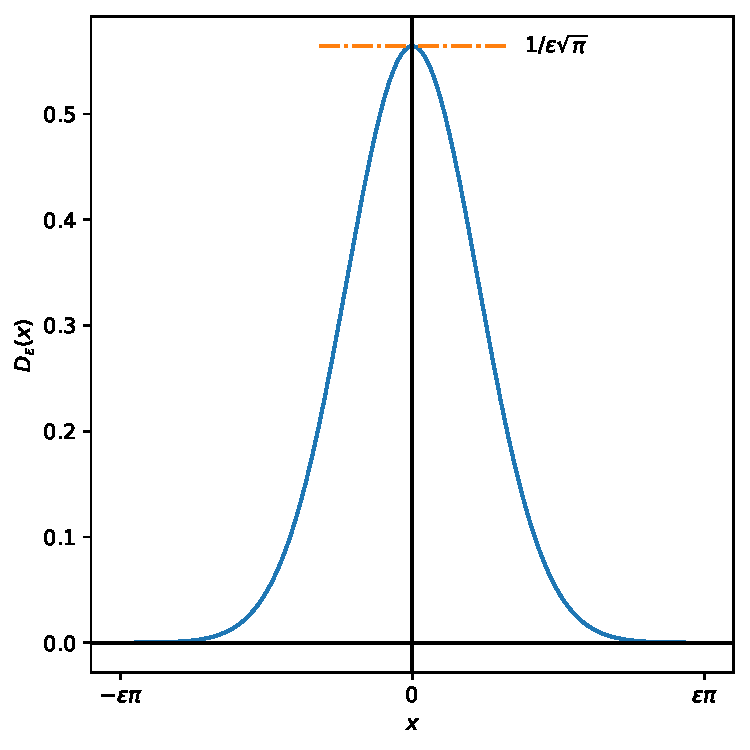
\includegraphics[width=5cm]{chapter1-delta-reps-exp.pdf}}
			\subfloat[]{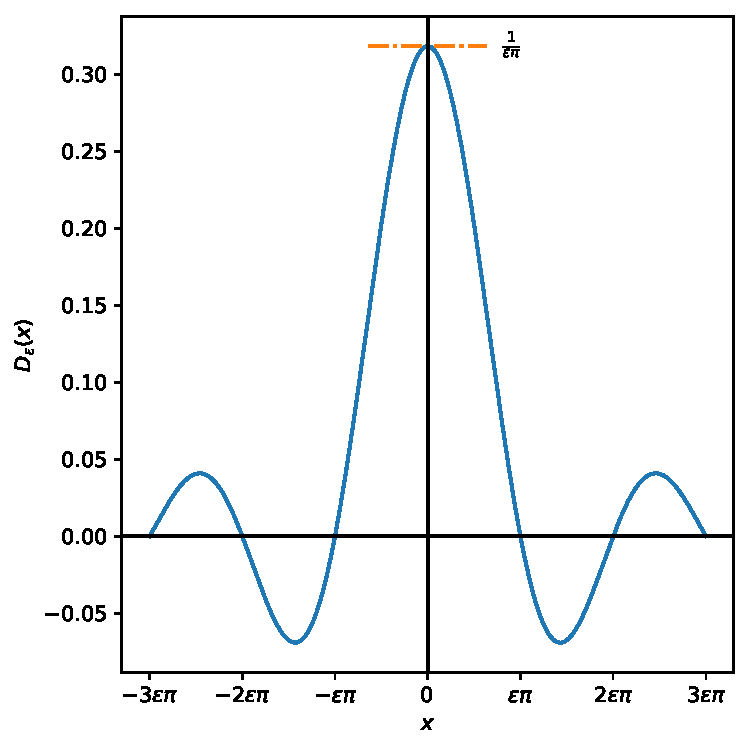
\includegraphics[width=5cm]{chapter1-delta-reps-sine.pdf}}
			\caption{Plot of function $D_\epsilon(x)$ for (a) equation (\ref{eqn.other-reps-exp}) (b) and equation (\ref{eqn.other-reps-sin})}
			\label{fig.cpt1.figure2}
		\end{figure}
		
		
		When plotted against $x$, the function has a peak at the origin. The peak has a height of $\frac{1}{\epsilon \sqrt{\pi}}$ and a width of order $\epsilon$ (exactly how the width is defined doesn't matter). So if $\epsilon$ is allowed to become very small, the peak becomes very tall and very narrow. Outside the peak the function becomes extremely small. Thus we have
		\begin{equation}
		\delta(x) = \lim\limits_{\epsilon \rightarrow 0}\frac{1}{\epsilon \sqrt{\pi}} e^{-x^2/\epsilon^2}
		\end{equation}
		
		%% proof
		
		\item
		Consider another function
		\begin{equation}
			D_\epsilon(x) = \frac{1}{\pi} \frac{\sin(x/\epsilon)}{x} \ \ \ \ (\epsilon > 0)
			\label{eqn.other-reps-sin}
		\end{equation} 
		

		
		For any value of the parameter $\epsilon$ we have 
		\begin{equation}
			\int_{-\infty}^{\infty} D_\epsilon(x) dx = 1
		\end{equation}
		A plot of the function $D_\epsilon(x)$ shows that it has the value $\frac{1}{\epsilon \pi}$ at $x=0$ and it oscillates with decreasing amplitude as $|x|$ increases. The width of the central maxima is of the order of $\epsilon$ and the period of oscillation with respect to $x$ is $2 \pi \epsilon$.\\
		Thus the limit of this function as $\epsilon \rightarrow 0 $ has all the properties of the delta function : it becomes infinitely large at $x=0$, it has unit integral, and infinitely rapid oscillations as $|x|$ increases means that the entire contribution to an integral containing this function comes from an infinitesimal neighborhood of $x=0$.\\
		We can therefore write,
		\begin{equation}
			\delta(x) = \lim\limits_{\epsilon \rightarrow 0} \frac{1}{\pi} \frac{\sin(x/\epsilon)}{x}
		\end{equation}

		\item
		We can also show that
		\begin{eqnarray}
			\delta(x) &= \lim\limits_{\epsilon \rightarrow 0} \frac{1}{2\epsilon} e^{-|x| / \epsilon} \\
			\delta(x) &= \lim\limits_{\epsilon \rightarrow 0} \frac{1}{\pi} \frac{\epsilon}{x^2 + \epsilon^2} \\
			\delta(x) &= \lim\limits_{\epsilon \rightarrow 0} \frac{\epsilon}{\pi} \frac{\sin^2(x/\epsilon)}{x^2}
		\end{eqnarray}
		
		\end{enumerate}	
	\section{Properties of the delta function}
		It is important to note that, because of its singular $@@@@@@$ , the $\delta$ function cannot be the end result of a calculation, and has meaning only so long as a subsequent integral over its argument is carried out. With this understanding we can write down some relations between delta functions.
		\begin{enumerate}[label=\textbf{Property \ \arabic*},start=1]
			\item 
			The delta function is a even function
			\begin{equation}
				\delta(-x) = \delta(x)
			\end{equation}
			
			\item
			\begin{equation}
				x \delta(x) = 0
			\end{equation}
			
			\item
			\begin{equation}
			\delta(a x) = \frac{1}{|a|} \delta(x)
			\end{equation}
			proof: Consider the integral
			\begin{equation}
				I = \int_{-\infty}^{\infty} \delta(a x) f(x) dx
			\end{equation}
			Since the delta function is even in its argument, it doesn't matter if we replace $a$ by $|a|$ in the argument. Thus
			\begin{equation}
				I = \int_{-\infty}^{\infty} \delta(|a| x) f(x) dx
			\end{equation}
			Making the change in variable $ y = |a| x$ we have,
			\begin{eqnarray}
				I &= \frac{1}{|a|}\int_{-\infty}^{\infty} \delta(y) f(y/|a|) dx \nonumber \\
				&= \frac{1}{|a|} f(0) \nonumber
			\end{eqnarray}			
			or
			\begin{equation}
				\int_{-\infty}^{\infty} \delta(a x) f(x) dx = \frac{1}{|a|} \int_{-\infty}^{\infty} \delta(x) f(x) dx
			\end{equation}
			or
			\begin{equation}
				\delta(a x) = \frac{1}{|a|} \delta(x)
			\end{equation}
			
			
			\item
			More generally
			\begin{equation}
				\delta(\phi(x)) = \sum_{i} \frac{\delta(x - x_i)}{\left|\frac{\partial\phi}{\partial x}\right|_{x_i}}
			\end{equation}
			where the sum sums over the $x_i$'s which are simple roots of $\phi(x)$.
			
			proof : let $x_1 , x_2, \ldots , x_N$ be the simple roots of $\phi(x)$,
			
			%figure
			
			In the neighborhood of any one of the simple roots $x_i$, we can write
			\begin{equation}
				\phi(x) = (x - x_i) \psi(x)
			\end{equation}
			where $\psi(x_i) \neq 0$. We have
			\begin{equation}
				\psi(x_i) = \left|\frac{\partial \phi(x)}{\partial x} \right|_{x=x_i}
			\end{equation}
			Now, consider the integral
			\begin{eqnarray}
				I &= \int_{-\infty}^{\infty} \delta(\phi(x)) f(x) dx  \nonumber \\
				&= \sum_{i=1}^{N} \int_{x_i - \epsilon}^{x_i + \epsilon} \delta[(x-x_i) \psi(x_i)] f(x) dx \nonumber \\
				&= \sum_{i=1}^{N} \frac{1}{|\psi(x_i)|}\int_{x_i - \epsilon}^{x_i + \epsilon} \delta(x-x_i) f(x) dx \nonumber \\
				&= \sum_{i=1}^{N} \frac{1}{ \left|\frac{\partial \phi(x)}{\partial x} \right|_{x=x_i}}\int_{-\infty}^{\infty} \delta(x-x_i) f(x) dx \nonumber \\
				&= \sum_{i=1}^{N} \frac{1}{ \left|\frac{\partial \phi}{\partial x} \right|_{x=x_i}} f(x_i) \nonumber
			\end{eqnarray}
			The above result is obtained if we write
			\begin{equation}
				\delta(\phi(x)) = \sum_{i=1}^{N} \frac{\delta(x - x_i)}{\left|\frac{\partial \phi}{\partial x}\right|_{x=x_i}}
			\end{equation}
			
			
			\item
			A frequently used example of the above result is
			\begin{equation}
				\delta(x^2 - a^2) = \frac{1}{2 a} \delta(x - a) + \frac{1}{2 a} \delta(x + a) \ \ \ \ (a > 0)
			\end{equation}
			
			Here
			\begin{equation}
				\phi(x) = x^2 - a^2 = (x-a)(x+a)
			\end{equation}
				The two simple roots of $\phi(x)$ are at $x=a $ and $x=-a$. Now
				\begin{eqnarray}
					\left|\frac{\partial \phi}{\partial x}\right|_{x=a} = \left|2 x\right|_{x=a} = 2a  \\
					\left|\frac{\partial \phi}{\partial x}\right|_{x=a} = \left|-2 x\right|_{x=-a} = 2a 
				\end{eqnarray}
				$\therefore$ The above result follows.
				
				\item
				\begin{equation}
					f(x) \delta(x-a) = f(a) \delta(x-a)
				\end{equation}

				\item
				\begin{equation}
					\int \delta(x-y) \delta(y-a) dy = \delta(x-a)
				\end{equation}
				
			
		\end{enumerate}
		
		\subsection{Notes}
		\begin{enumerate}[label=\textbf{Note : \ \arabic*},start=1]
			\item 
			We have the identity
			\begin{equation}
				x\delta(x) = 0
			\end{equation}
			The converse is also true and it can be shown that the equation
			\begin{equation}
				x u(x) = 0
			\end{equation}
			has the general solution
			\begin{equation}
				u(x) = c \delta(x)
			\end{equation}
			
			
			\item
			We will now prove an identity which is particularly useful in Quantum Mechanics.
			\begin{equation}
				\lim\limits_{\epsilon \rightarrow 0^+} \int_{-\infty}^{\infty} \frac{1}{x \pm \imath \epsilon} f(x) dx = \rho \int_{-\infty}^{\infty} \frac{dx}{x}f(x) \mp \imath\pi f(0)
			\end{equation}
			or in short
			\begin{equation}
				\lim\limits_{\epsilon \rightarrow 0^+} \frac{1}{x \pm \imath \epsilon} = \rho(\frac{1}{x}) \mp \imath \pi \delta(x)
			\end{equation}
			Where it is understood that the second of these two equations have meaning only within an integral.\\
			The symbol $\rho$ means principle part of an integral where the integral has a single pole. The principle part is defined as
			\begin{equation}
				\rho \int_{-A}^{B} \frac{dx}{x} f(x) dx = \lim\limits_{\eta \rightarrow 0^+} \left[\int_{-A}^{-\eta} + \int_{\eta}^{B}\right] \frac{dx}{x} f(x)
			\end{equation}
			\textbf{proof :}
			\begin{equation}
				\frac{1}{x \pm \imath \epsilon} = \frac{x \mp \imath\epsilon}{x^2 + \epsilon^2} = \frac{x}{x^2 + \epsilon^2} \mp \frac{\imath \epsilon}{x^2 + \epsilon^2}
			\end{equation}
			Now we have
			\begin{eqnarray}\label{eqn:1}
				\lim\limits_{\epsilon \rightarrow 0^+} \frac{1}{\pi} \frac{\epsilon}{x^2 + \epsilon^2} &= \delta(x) \nonumber \\
				\lim\limits_{\epsilon \rightarrow 0^+} (\mp) \imath \frac{\epsilon}{x^2 + \epsilon^2} &= \mp \imath \pi \delta(x)
			\end{eqnarray}
			Now consider the first term on the right hand side of equation  \ref{eqn:1}. We multiply this term by a function $f(x)$ which is regular at the origin and then integrate over $x$. We get
			\begin{equation}\label{eqn:2}
				\lim\limits_{\epsilon \rightarrow 0^+} \int_{-\infty}^{\infty} \frac{x f(x)}{x^2 + \epsilon^2} dx
				=\lim\limits_{\epsilon \rightarrow 0^+}\left[
				\lim\limits_{\eta \rightarrow 0^+}\left[ \int_{-\infty}^{-\eta} \frac{x f(x)}{x^2 + \epsilon^2}
				+\int_{-\eta}^{\eta} \frac{x f(x)}{x^2 + \epsilon^2}
				+\int_{\eta}^{\infty} \frac{x f(x)}{x^2 + \epsilon^2} dx\right]\right]
			\end{equation}
			Note that we take the limit over $\eta$ first and then we take the limit over $\epsilon$. Consider now the second integral above
			\begin{equation} 
				\lim\limits_{\eta \rightarrow 0^+} \int_{-\eta}^{+\eta} \frac{x f(x)}{x^2 + \epsilon^2} = f(0) \lim\limits_{\eta \rightarrow 0^+} \frac{1}{2}  \left[\ln({x^2 + \epsilon^2}
				)\right]_{x=-\eta}^{x=\eta} = 0
			\end{equation}
			If we now reverse the order of the evaluation of limits in equation \ref{eqn:2}, the $\epsilon \rightarrow 0$ limit causes no difficulties in the other two integrals.
			Thus we have
			\begin{eqnarray}
				&\lim\limits_{\epsilon \rightarrow 0^+} \int_{-\infty}^{\infty} \frac{x dx}{x^2 + \epsilon^2} f(x)\nonumber \\
				 = &\lim\limits_{\eta \rightarrow 0^+} \lim\limits_{\epsilon \rightarrow 0^+} \left[\int_{-\infty}^{-\eta} + \int_{\eta}^{\infty}\right] \frac{x dx}{x^2 + \epsilon^2} f(x) \nonumber \\
				 = &\lim\limits_{\eta \rightarrow 0^+} \left[\int_{-\infty}^{-\eta} + \int_{\eta}^{\infty}\right] \frac{dx}{x} f(x) \nonumber\\
				 = & \rho \int_{-\infty}^{\infty} \frac{1}{x} f(x) dx \nonumber
			\end{eqnarray}
			This establishes the identity.
		\end{enumerate}
		
	\section{Derivatives of the delta function}
		One may define the derivative $\delta^\prime(x)$ of the delta function. When $\epsilon$ is small, the derivative of $D_\epsilon(x)$ has two peaks close to the origin, one peak is positive and the other is negative as drawn in the figure below
		
		\begin{figure}
			\centering
			\subfloat[]{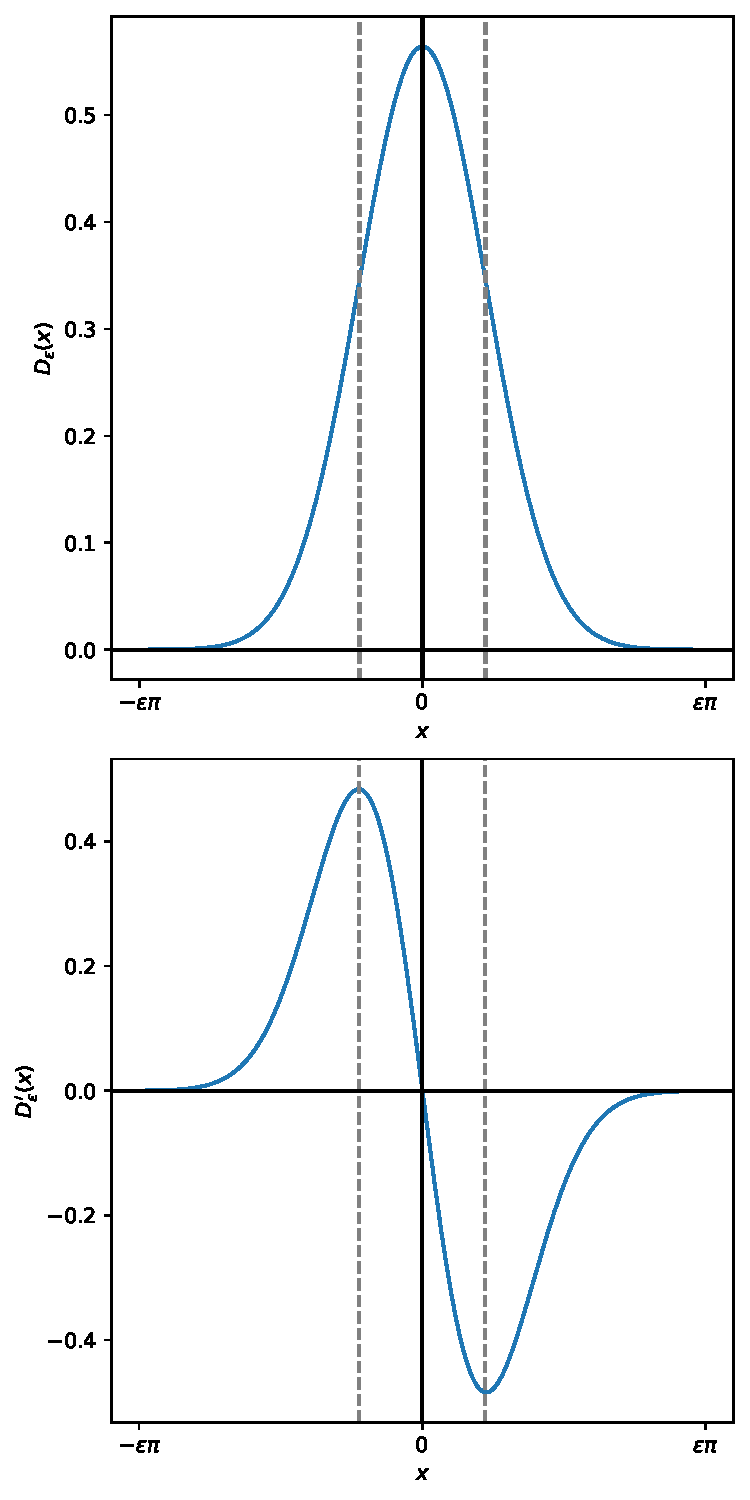
\includegraphics[height=8cm,width=5cm]{chapter1-delta-reps-exp-derivative.pdf}}
			\caption{(a) Derivative of Delta Function}
			\label{}
		\end{figure}
		% figure
		
		
		As $\epsilon \rightarrow 0$, each of these peaks becomes very narrow and very tall, and two peaks each approach very close to the origin. \\
		Now the integration by parts gives
		\begin{equation}
			\int_{-\infty}^{\infty} dx D_\epsilon^\prime(x) f(x) = \left[D_\epsilon(x) f(x)\right]_{-\infty}^{\infty} - \int_{-\infty}^{\infty} dx D_\epsilon(x) f^\prime(x)
		\end{equation}
		Because $D_\epsilon(x)$ tens to zero as $x \rightarrow \pm \infty$, the first term on the right hand side vanishes unless $f(x)$ $@@@@@@@$ violently at infinity. So by letting $\epsilon \rightarrow 0$, we arrive at the definition of $\delta^\prime(x)$
		\begin{equation}\label{eqn:3}
			\int_{-\infty}^{\infty} \delta^\prime(x) f(x) dx = - \int_{-\infty}^{\infty} \delta(x) f^\prime(x) dx = - f^\prime(0)
		\end{equation}
		From this we immediately get
		\begin{equation}
			x \delta^\prime(x) = -\delta(x)
		\end{equation}
		Conversely, it can be shown that the general solution of the equation
		\begin{equation}
			x u(x) = \delta(x)
		\end{equation}
		can be written as
		\begin{equation}
			u(x) = -\delta^\prime(x) + c \delta(x)
		\end{equation}
		Where the second term arises from the homogeneous equation $x \delta(x) = 0$.
		From equation  \ref{eqn:3}  it also follows that 
		\begin{equation}
			\delta^\prime(-x) = - \delta^\prime(x)
		\end{equation}
		The $n^{th}$ order derivative of $\delta(x)$ can be defined in the same way. We find
		\begin{equation}
			\int_{-\infty}^{\infty} \delta^{(n)}(x) f(x) dx = (-1)^{n} f(0)
		\end{equation}
		We can prove the following properties:
		\begin{eqnarray}
			\delta^{(m)}(x) &= (-1)^m \delta^{(m)} (-x) \\
			x^{m+1} \delta^{(m)}(x) &= 0 \\
			x\delta^{(m)}(x) &= -m \delta^{(m-1)} (x)
		\end{eqnarray}
		
		
	\section{Integration of the delta function}
		Consider the indefinite integral
		\begin{equation}\label{eqn:4}
			\Theta_\epsilon(x) = \int_{-\infty}^{x}  D_\epsilon(y) dy
		\end{equation}
		A graph of $\Theta_\epsilon(x)$ vs $x$ is shown below
		
		%figure
		
		As $\epsilon \rightarrow 0$, the step in the function $\Theta_\epsilon(x)$ gets progressively steeper, until, finally, the function changes abruptly from $0$ to $1$ at $x=0$.
		Thus taking the limit $\epsilon \rightarrow 0$ in equation \ref{eqn:4} we have
		\begin{equation}\label{eqn:5}
			\Theta(x) = \int_{-\infty}^{x} \delta(x) dx
		\end{equation}
		Where
		\begin{equation}
			\Theta(x) = 
			\begin{cases}
				1 \ \ \text{for} \ \ x > 0 \\
				0 \ \ \text{for} \ \ x < 0
			\end{cases}
		\end{equation}
		If we differentiate equation \ref{eqn:5} with respect to $x$,\\
		we get
		\begin{equation}
			\frac{d \Theta(x)}{dx} = \delta(x)
		\end{equation}
		
	\section{Three - dimensional delta function}
		\begin{equation}
			\delta(\vec{r}) _=^{def} \delta(x) \delta(y) \delta(z)
		\end{equation}
		In other words, $\delta(\vec{r})$ is zero if any of the coordinates $x, y, z$ is not equal to zero and $\delta(\vec{r})$ tends to infinity at the origin, i.e., when $x=0, y=0, z=0$, such that 
		\begin{equation}
			\int_{volume} \delta(\vec{r}) d^3 r = 1
		\end{equation}
		if the volume of the integration contains the origin. We also have
		\begin{equation}
			\int \delta(\vec{r}) f(\vec{r}) d^3 r = f(0)
		\end{equation}
		where again the volume of the integration includes the origin.
		\textbf{Note:}
		\begin{eqnarray}
			\delta(\vec{r} - \vec{r^\prime}) &= \delta(x - x^\prime) \delta(y - y^\prime) \delta(z-z^\prime) \\
			\int_{v}\delta(\vec{r} - \vec{r^\prime}) d^3r &= 1
		\end{eqnarray}
		where the volume of integration includes the point $\vec{r}^\prime$. Otherwise the integral is zero.
		\begin{equation}
			\int_{v}\delta(\vec{r} - \vec{r^\prime}) f(\vec{r}) d^3r = f(\vec{r^\prime})
		\end{equation}
		if V includes the point $\vec{r^\prime}$.
		
		\textbf{A useful formula}
		Consider the integral
		\begin{eqnarray}
			\int_{-\infty}^{\infty} e^{\imath k x} dx 
			&= \lim\limits_{L \rightarrow \infty} \int_{-L}^{L} e^{\imath k x} dx \nonumber \\
			&= \lim\limits_{L \rightarrow \infty} \frac{1}{\imath k} \left(e^{\imath k L} - e^{-\imath k L}\right) \nonumber \\
			&= \lim\limits_{L \rightarrow \infty} \frac{2}{k} \left(\frac{e^{\imath k L} - e^{-\imath k L}}{2\imath}\right) \nonumber \\
			&= \lim\limits_{L \rightarrow \infty} \frac{2}{k} \sin(k L) \nonumber \\
			&= 2\pi \lim\limits_{L \rightarrow \infty} \frac{\sin(k L
				)}{\pi k} \nonumber \\
			&= 2\pi \delta(k)
		\end{eqnarray}
		using 
		\begin{equation}
			\lim\limits_{\epsilon \rightarrow 0} \frac{\sin(x /\epsilon
				)}{\pi x} = \delta(x)
		\end{equation}
		Thus
		\begin{equation}\label{eqn:6}
			\int_{-\infty}^{\infty} e^{\imath k x} dx = 2\pi \delta(k)
		\end{equation}
		In equation \ref{eqn:6} if we integrate with respect to $k$, we would have $delta(x)$ on the right hand side,
	
	%%%%%%%%%%%%%%%%%%%%%%%%%%%% equation number
	
		\begin{equation}\label{eqn:100}
		\int_{-\infty}^{\infty} e^{\imath k x} dk = 2\pi \delta(x)
		\end{equation}
		Also note that in equation \ref{eqn:6} we are integrating over its full range of values. Making a change of variable $x \rightarrow -x$ does not change the value of the integral. Hence we also have
		
		\begin{equation}\label{eqn:101}
		\int_{-\infty}^{\infty} e^{-\imath k x} dx = 2\pi \delta(k)
		\end{equation}
		Similarly, in equation \ref{eqn:100} making the change $k \rightarrow -k$, doesn't change the value of the integral. So we could also write
		\begin{equation}\label{eqn:102}
		\int_{-\infty}^{\infty} e^{-\imath k x} dk = 2\pi \delta(x)
		\end{equation}
		
		Thus in summary
		\begin{eqnarray}\label{eqn:103-104}
			\int_{\pm \infty}^{\infty} e^{-\imath k x} dx &= 2\pi \delta(k)
			\int_{\pm \infty}^{\infty} e^{-\imath k x} dk &= 2\pi \delta(x)
		\end{eqnarray}
		In three dimensions
		\begin{eqnarray}\label{eqn:105-107}
			\int_{all\ space} e^{\pm \imath \vec{k} . \vec{r}} d^3\vec{r} &= (2\pi)^3 \delta(\vec{k}) \\
			\int_{all\ space} e^{\pm \imath (\vec{k} - \vec{k^\prime}) . \vec{r}} d^3\vec{r} &= (2\pi)^3 \delta(\vec{k} - \vec{k^\prime}) \\
			\int_{all\ space} e^{\pm \imath \vec{k} . (\vec{r} - \vec{r^\prime})} d^3\vec{r} &= (2\pi)^3 \delta(\vec{r} - \vec{r^\prime}) \\
		\end{eqnarray}
		
	\section{Fourier Transformation}
		We can always express a function $f(x)$ in the form
		\begin{eqnarray}\label{eqn:108}
			f(x) = \int_{-\infty}^{\infty} e^{\imath k x} \tilde{f}(k) dk
		\end{eqnarray}
		where $\tilde{f}(k)$ is a function of $k$, called the fourier transform of $f(x)$. From eqnarray \ref{eqn:108} we can write
		
		\begin{eqnarray}\label{eqn:109}
			\int_{-\infty}^{\infty} e^{-\imath k^\prime x} f(x) dx 
			&= \int_{-\infty}^{\infty} \int_{-\infty}^{\infty} e^{i(k-k^\prime) x} \tilde{f}(k) dk dk^\prime \nonumber \\
			&= 2 \pi \int_{-\infty}^{\infty} \delta(k-k^\prime) \tilde{f}(k) dk \nonumber \\
			&= 2\pi \tilde{f}(k^\prime) 
		\end{eqnarray}
		
		Thus
		\begin{eqnarray}\label{eqn:110}
			\tilde{f}(k) = \frac{1}{2\pi} \int_{-\infty}^{\infty} e^{-\imath k x} f(x) dx
		\end{eqnarray}
		Thus functions $f(x)$ and $\tilde{f}(k)$ are Fourier transform of each other. We can write eqnarray \ref{eqn:108} and \ref{eqn:110} in a more symmetrical fashion as follows:
		\begin{eqnarray}\label{eqn:111}
		f(x) = \frac{1}{\sqrt{2\pi}} \int_{-\infty}^{\infty} e^{\imath k x} \tilde{f}(k) dk
		\end{eqnarray}
		\begin{eqnarray}\label{eqn:112}
			\tilde{f}(k) = \frac{1}{\sqrt{2\pi}} \int_{-\infty}^{\infty} e^{-\imath k x} f(x) dx
		\end{eqnarray}
		In three dimension, we can write
		\begin{eqnarray}\label{eqn:113}
			f(\vec{r}) = \frac{1}{(2\pi)^{3/2}} \int_{all\ k-space} e^{i \vec{k} . \vec{r}} \tilde{f}(\vec{k}) d^3k
		\end{eqnarray}
		multiplying eqnarray \ref{eqn:113} by $e^{-i\vec{k^\prime} . \vec{r}} $ and integrating over $\vec{r}$, we have
		\begin{eqnarray}\label{eqn:114}
			\int_{all\ space} e^{-i\vec{k^\prime} . \vec{r}} f(\vec{r}) d^3 r
			&= \frac{1}{(2\pi)^{3/2}} \int d^3 r \int d^3 k \ e^{i (\vec{k} - \vec{k^\prime}). \vec{r}} \tilde{f}(\vec{k}) \nonumber \\
			&= \frac{1}{(2\pi)^{3/2}} \int d^3 k (2\pi)^3 \delta(\vec{k} - \vec{k^\prime}) \tilde{f}(\vec{k}) \nonumber \\
			&= \frac{1}{(2\pi)^{-3/2}} \tilde{f}(\vec{k^\prime})
		\end{eqnarray}
		
		Therefore
		\begin{eqnarray}\label{eqn:115}
			\tilde{f}(\vec{k}) = \frac{1}{(2\pi)^{3/2}} \int e^{-i\vec{k} . \vec{r}} f(\vec{r}) d^3 r
		\end{eqnarray}
		Thus we can write 
		\begin{eqnarray}\label{eqn:116}
		f(\vec{r}) = \frac{1}{(2\pi)^{3/2}} \int e^{i\vec{k} . \vec{r}} \tilde{f}(\vec{k}) d^3 k
		\end{eqnarray}
		\begin{eqnarray}\label{eqn:117}
		\tilde{f}(\vec{k}) = \frac{1}{(2\pi)^{3/2}} \int e^{-i\vec{k} . \vec{r}} f(\vec{r}) d^3 r
		\end{eqnarray}
		
		\textbf{Parseval's Identity:}\\
		We can now  prove the important identity
		\begin{eqnarray}\label{eqn:118}
			\int |f(\vec{r})|^2 d^3r = \int |\tilde{f}(\vec{k})|^2 d^3k
		\end{eqnarray}
		proof:
		\begin{eqnarray}
			\int |f(\vec{r})|^2 d^3r
			&= \int f(\vec{r}) f^*(\vec{r}) d^3r \nonumber \\
			&= \int d^3r \frac{1}{(2\pi)^{3/2}} \int e^{\imath\vec{k} . \vec{r}} \tilde{f}(\vec{k}) d^3k \frac{1}{(2\pi)^{3/2}} \int e^{-\imath\vec{k^\prime} . \vec{r}} \tilde{f}^*(\vec{k^\prime}) d^3k^\prime \nonumber \\
			&= \frac{1}{(2\pi)^3} \int d^3k\ d^3k^\prime \tilde{f}(\vec{k}) \tilde{f}^*(\vec{k^\prime}) \int d^3r \ e^{\imath(\vec{k} - \vec{k^\prime}).\vec{r}} \nonumber \\
			&= \frac{1}{(2\pi)^3} \int d^3k\ d^3k^\prime \tilde{f}(\vec{k}) \tilde{f}^*(\vec{k^\prime}) (2\pi)^3 \delta(\vec{k} - \vec{k^\prime}) \nonumber \\
			&= \int d^3k\ \tilde{f}(\vec{k}) \tilde{f}^*(\vec{k}) \nonumber \\
			&= \int |\tilde{f}(\vec{k})|^2 d^3k
		\end{eqnarray}
		
		
		
		
		